% !TEX root = ../main.tex
\chapter{Дослідження стійкості}
Дослідимо стійкість контура цифрового керування
з передаточною функцією об'єкта $W_O(s) = \frac{k e^{-\tau s}}{T_1 s + 1}$
та ПІ-регулятором, що має дискретну передаточну функцію
$W_p(z) = K_p \left(1 + \frac{T_0}{T_I \left(1 - z^{-1}\right)}\right)$.
Взявши період квантування $T_0 = 1.5430$, отриманий методом Джурі
у пункті \ref{jury_for_stability}, за 
формулами \eqref{K_p_opt__direct} та \eqref{T_I_opt__direct}
при $\lambda = \frac{1}{T_1}$
визначимо оптимальні настройки ПІ-регулятора :
\begin{gather*}
    K_{p_{\text{опт}}} = 34.2342, T_{I_{\text{опт}}} = 0.0740
\end{gather*}

\section{Критерій Гурвіца}
Розрахунок стійкості замкненої системи цифрового керування 
проведемо за послідовністю, наведеною у методичних рекомендаціях.

а)\; $d$ -- ціле число від ділення часу запізнення на період квантування $T_0$, воно дорівнює 9.

б)\; За формулою \eqref{transfer_function_for_stability} обчислимо дискретну передаточну функцію приведеної неперервної частини:
\begin{gather*}
    W_\text{п}(z) = \frac{
        0.37311 z^{-10} + 0.02884 z^{-11}
    }{
        1 - e^{-0.04409} z^{-1}
    }
\end{gather*}

в)\; Визначимо характеристичне рівняння замкненого контуру:
\begin{gather}
    1 + W_p(z)W_\text{п}(z) = 0 \Leftrightarrow \nonumber \\ \Leftrightarrow
    z^{12} -1.95687 z^{11} + 0.95687 z^10 + 0.02881 z^2 -0.02537 z -0.00213 = 0 \label{hurwitz_char_pol}
\end{gather}

г)\; Застосуємо $w$-перетворення до \eqref{hurwitz_char_pol}, підставивши $z = \frac{1+w}{1-w}$:
\begin{gather}
    3.96579 w^{12} + 38.76510 w^{11} + 178.70561 w^{10} + 470.05698 w^9 + 835.79917 w^8 + \nonumber \\ 
    + 1004.10086 w^7 + 839.23167 w^6 + 494.18403 w^5 + 181.65973 w^4 + 45.12629 w^3 + \nonumber \\
    + 4.26842 w^2 + 0.13504 w + 0.00131 = 0 \label{hurwitz_char_pol_in_w}
\end{gather}

д)\; Складемо для полінома з \eqref{hurwitz_char_pol_in_w} матрицю Гурвіца та перевіримо додатність усіх діагональних мінорів. Матриця Гурвіца має вигляд

\begin{gather*}
    \mbox{\tiny
    $
    \left[\begin{array}{cccccccccccc}
        38.7651 & 470.057 & 1004.1009 & 494.184 & 45.1263 & 0.135 & 0.0 & 0.0 & 0.0 & 0.0 & 0.0 & 0.0 \\
        3.9658 & 178.7056 & 835.7992 & 839.2317 & 181.6597 & 4.2684 & 0.0013 & 0.0 & 0.0 & 0.0 & 0.0 & 0.0 
        \\0.0 & 38.7651 & 470.057 & 1004.1009 & 494.184 & 45.1263 & 0.135 & 0.0 & 0.0 & 0.0 & 0.0 & 0.0 
        \\0.0 & 3.9658 & 178.7056 & 835.7992 & 839.2317 & 181.6597 & 4.2684 & 0.0013 & 0.0 & 0.0 & 0.0 & 0.0 
        \\0.0 & 0.0 & 38.7651 & 470.057 & 1004.1009 & 494.184 & 45.1263 & 0.135 & 0.0 & 0.0 & 0.0 & 0.0 
        \\0.0 & 0.0 & 3.9658 & 178.7056 & 835.7992 & 839.2317 & 181.6597 & 4.2684 & 0.0013 & 0.0 & 0.0 & 0.0 
        \\0.0 & 0.0 & 0.0 & 38.7651 & 470.057 & 1004.1009 & 494.184 & 45.1263 & 0.135 & 0.0 & 0.0 & 0.0 
        \\0.0 & 0.0 & 0.0 & 3.9658 & 178.7056 & 835.7992 & 839.2317 & 181.6597 & 4.2684 & 0.0013 & 0.0 & 0.0 
        \\0.0 & 0.0 & 0.0 & 0.0 & 38.7651 & 470.057 & 1004.1009 & 494.184 & 45.1263 & 0.135 & 0.0 & 0.0 
        \\0.0 & 0.0 & 0.0 & 0.0 & 3.9658 & 178.7056 & 835.7992 & 839.2317 & 181.6597 & 4.2684 & 0.0013 & 0.0 
        \\0.0 & 0.0 & 0.0 & 0.0 & 0.0 & 38.7651 & 470.057 & 1004.1009 & 494.184 & 45.1263 & 0.135 & 0.0 
        \\0.0 & 0.0 & 0.0 & 0.0 & 0.0 & 3.9658 & 178.7056 & 835.7992 & 839.2317 & 181.6597 & 4.2684 & 0.0013
    \end{array}\right]
    $
    }
\end{gather*}
Комп'ютерне обчислення показує, що усі діагональні мінори є додатними. Це означає, що усі корені рівняння \eqref{hurwitz_char_pol_in_w}
мають від'ємні дійсні частини, а отже, усі корені рівняння \eqref{hurwitz_char_pol} за модулем менше одиниці, що свідчить про стійкість
контуру, що розглядається.

\section{Аналог критерію Михайлова}
Для застосування аналогу критерію Михайлова розглянемо поліном з рівняння \eqref{hurwitz_char_pol} (який одразу записано з коефіцієнтом 1 перед старшим степенем).
Підставимо $z = e^{j \omega T_0} = \cos \left(\omega T_0\right) + j \sin \left(\omega T_0\right)$:
\begin{gather*}
    F(z) = z^n + a_{n-1} z^{n-1} + \dots + a_1 z + a_0 \Rightarrow \\
    \Rightarrow F\left(e^{j \omega T_0}\right) = 
    e^{j \omega n T_0} + a_{n-1} e^{j \omega (n-1) T_0} + \dots + a_1 e^{j \omega T_0} + a_0 = \\ =
    \left[
        \cos \left(\omega n T_0\right) + a_{n-1} \cos \left(\omega (n-1) T_0\right) + \dots + a_1 \cos \left(\omega T_0\right) + a_0
    \right] + \\ +
    j \left[
        \sin \left(\omega n T_0\right) + a_{n-1} \sin \left(\omega (n-1) T_0\right) + \dots + a_1 \sin \left(\omega T_0\right)
    \right] = u (\omega) + j v (\omega)
\end{gather*}
Побудуємо годограф $F\left(e^{j \omega T_0}\right)$ при зміні частоти в межах $0 \leq \omega \leq \frac{\pi}{T_0}$:
\begin{center}
    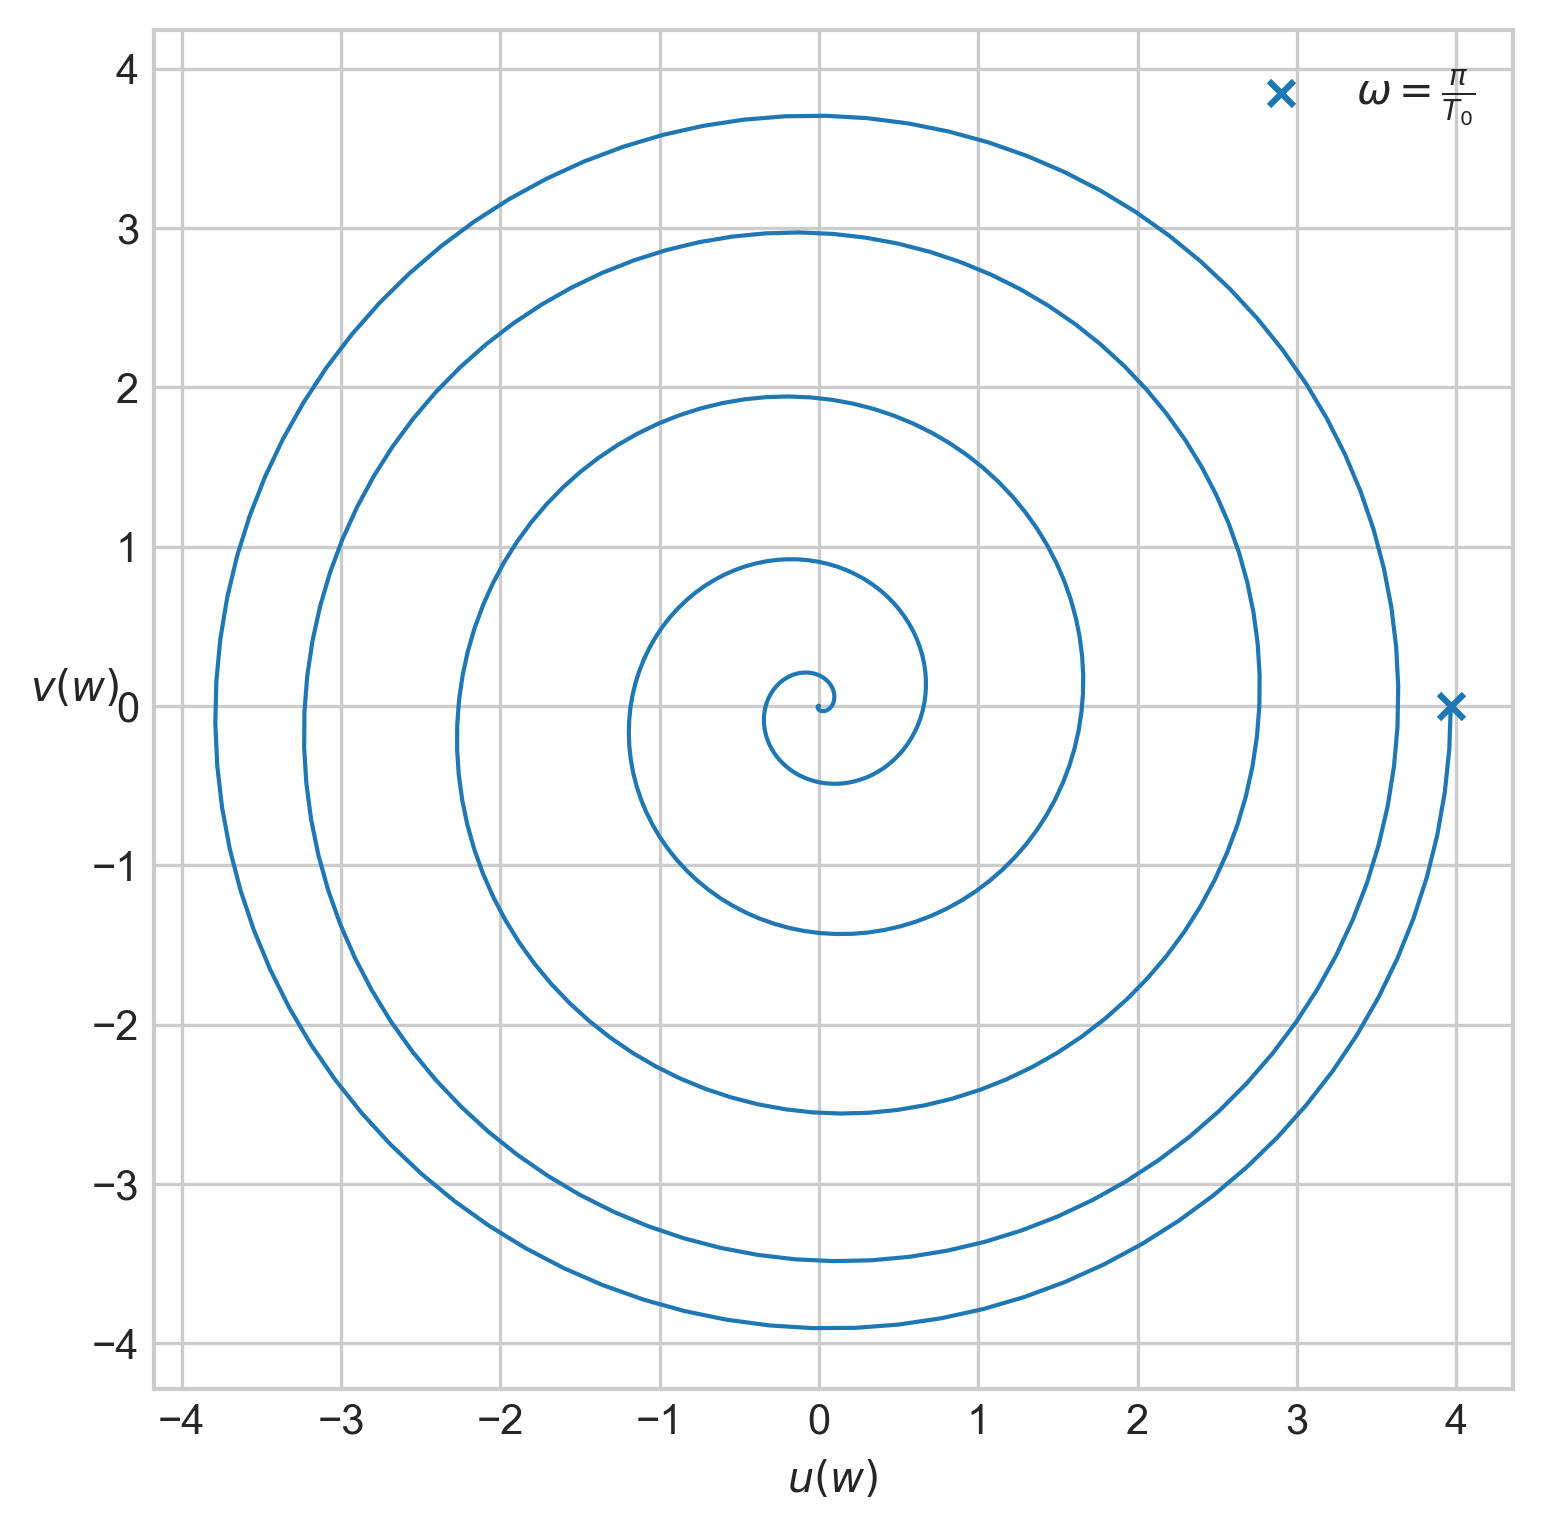
\includegraphics{pics/hodograph.png}
\end{center}
Можна порахувати, що годограф пройшов $2\cdot 12 = 24$ квадранти, тому контур є стійким.